\documentclass[a4paper,11pt]{article}

% --- Pakete ---
\usepackage[utf8]{inputenc}
\usepackage[T1]{fontenc}
\usepackage{geometry}
\geometry{margin=2.5cm}
\usepackage{enumitem}
\usepackage{tabularx}
\usepackage{booktabs}
\usepackage{tikz}
\usetikzlibrary{arrows.meta, positioning}
\usepackage{graphicx}
\usepackage{titling}
\usepackage{parskip}
\usepackage{hyperref}
\hypersetup{colorlinks=true, urlcolor=blue, linkcolor=black}

% --- Titel ---
\title{\textbf{UART \\ \large Universal Asynchronous Receiver Transmitter}}
\author{Gabriel Djak}
\date{\today}

\begin{document}

\maketitle
\vspace{-0.8cm}

\section*{Was ist UART?}

UART steht für \textbf{U}niversal \textbf{A}synchronous \textbf{R}eceiver \textbf{T}ransmitter. Es handelt sich um einen Hardware-Baustein bzw. ein Protokoll zur \textbf{seriellen Datenübertragung} zwischen zwei Geräten -- Daten werden dabei Bit für Bit über eine Leitung gesendet, statt parallel über mehrere Leitungen gleichzeitig.

\subsection*{Wichtige Eigenschaften}

\begin{itemize}[leftmargin=1.5em]
    \item \textbf{Asynchron:} Es gibt kein gemeinsames Taktsignal (Clock) zwischen Sender und Empfänger. Beide Seiten müssen vorher auf dieselbe Übertragungsgeschwindigkeit (Baudrate, z.\,B. 9600, 115200 Baud) eingestellt sein.
    \item \textbf{Zwei Leitungen:} Typischerweise nur TX (Transmit/Senden) und RX (Receive/Empfangen), plus gemeinsame Masse (GND).
    \item \textbf{Punkt-zu-Punkt:} UART verbindet meist genau zwei Geräte miteinander (im Gegensatz z.\,B. zu I\textsuperscript{2}C oder CAN, die mehrere Geräte am selben Bus erlauben).
\end{itemize}

\section*{Aufbau eines UART-Frames}

Ein typisches UART-Frame besteht aus:

\begin{enumerate}[leftmargin=1.5em]
    \item \textbf{Startbit} (signalisiert Beginn der Übertragung)
    \item \textbf{Datenbits} (meist 5--9 Bit, üblich sind 8 Bit)
    \item \textbf{Optionales Paritätsbit} (zur Fehlererkennung)
    \item \textbf{Stoppbit(s)} (1 oder 2 Bit, signalisiert Ende)
\end{enumerate}

\begin{center}
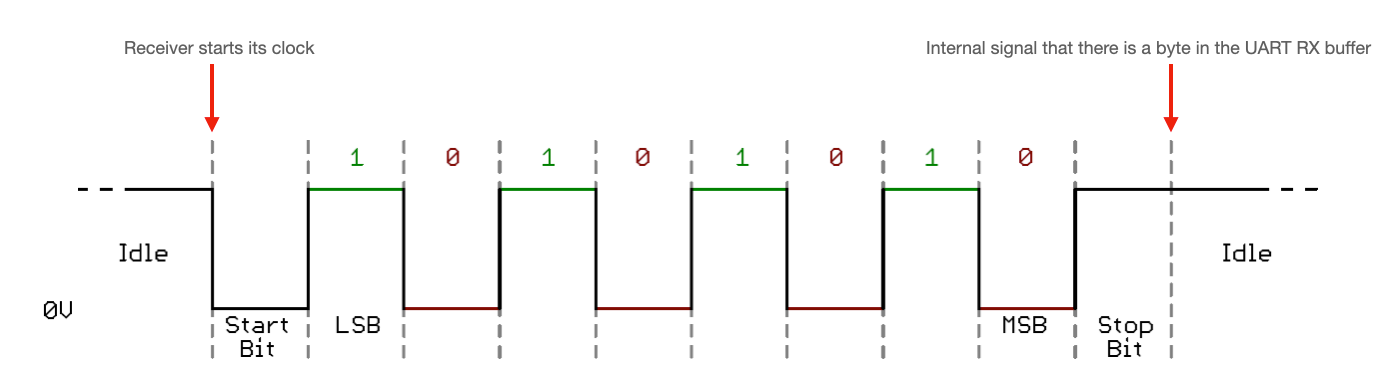
\includegraphics[width=0.75\textwidth]{uart_frame.png}
\end{center}

\section*{Verbindung zwischen zwei Teilnehmern}

Für eine UART-Verbindung reichen \textbf{3 Leitungen}: TX, RX und GND. Wichtig ist die \textbf{Kreuzung} von TX und RX:

\begin{itemize}[leftmargin=1.5em]
    \item TX (Transmit) von Gerät A geht zu RX (Receive) von Gerät B
    \item RX von Gerät A kommt von TX von Gerät B
    \item GND (Masse) muss unbedingt verbunden werden -- dient als gemeinsame Referenzspannung für die Signalpegel
\end{itemize}

\begin{center}
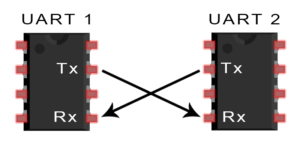
\includegraphics[width=0.4\textwidth]{uart_connection.png}
\end{center}

Wichtig: Die Spannungspegel beider Geräte müssen zueinander passen (z.\,B. 3{,}3\,V vs.\ 5\,V) -- bei Unterschieden ist ein Pegelwandler (Level Shifter) notwendig.

\section*{Beispiel: 3 Geräte mit UART-Schnittstelle}

\begin{enumerate}[leftmargin=1.5em]
    \item \textbf{GPS-Modul} (z.\,B. NEO-6M)
    \item \textbf{ESP32} (Mikrocontroller)
    \item \textbf{Bluetooth-Modul} (z.\,B. HC-05)
\end{enumerate}

Da UART nur Punkt-zu-Punkt funktioniert, nutzt man bei 3 Teilnehmern meist einen Mikrocontroller mit \textbf{mehreren Hardware-UARTs} (z.\,B. ESP32) als Zentrale, an die jeweils ein Peripheriegerät über eine eigene UART-Strecke angeschlossen wird.

\section*{Datenrate (Baudrate)}

UART als Standard schreibt \textbf{keine festen Baudraten} vor -- theoretisch ist jede Rate möglich, solange:

\begin{itemize}[leftmargin=1.5em]
    \item die Hardware (Baudratengenerator/Taktquelle) sie erzeugen kann,
    \item beide Kommunikationspartner exakt dieselbe Rate eingestellt haben,
    \item die Signalqualität (Leitungslänge, Störungen, Anstiegszeiten) sie noch sauber überträgt.
\end{itemize}

\subsection*{Typische (genormte) Baudraten}

\begin{center}
\begin{tabularx}{\textwidth}{@{}l X@{}}
\toprule
\textbf{Baudrate} & \textbf{Einsatzbereich} \\
\midrule
110, 300, 600 & historisch (alte Modems) \\
1200, 2400, 4800 & langsame/robuste Verbindungen \\
9600 & Klassiker, De-facto-Standard (Arduino-Default, viele Sensoren) \\
19200, 38400 & Debug, ältere Peripherie \\
57600 & häufig bei GPS-Modulen \\
115200 & Standard für Mikrocontroller-Debugging (ESP32, STM32, Arduino) \\
230400 & schnellere Konsolen/Logging \\
460800 & High-Speed-Anwendungen \\
921600 & z.\,B. ESP32-Flashen, schnelle Datenlogger \\
bis mehrere Mbit/s & spezielle High-Speed-UART-Peripherie \\
\bottomrule
\end{tabularx}
\end{center}

\bigskip
\noindent\rule{\textwidth}{0.4pt}

\noindent\textit{Zusammenfassung UART -- Gabriel Djak}

\end{document}